\documentclass[11pt]{article}
\usepackage[margin=1in]{geometry}
\usepackage{amsmath,amssymb}
\usepackage{booktabs}
\usepackage{graphicx}
\usepackage{float}
\usepackage{hyperref}

\title{Data 37711 Homework 3 --- Problem 3\\
\large Generalization of gradient boosting as the number of trees grows}
\author{Yiwen Chen}
\date{}

\begin{document}
\maketitle

\paragraph{Setup.} The code is in \texttt{problem3.py}. In both \texttt{dset0.csv} and
\texttt{dset1.csv}, the first column is a binary label and the other five columns are covariates.
Each file has $n=500$ rows. The positive rate is $42.6\%$ in dset0 and $45.4\%$ in dset1. I use
\texttt{sklearn.ensemble.GradientBoostingClassifier} with its defaults: log-loss, learning rate
$0.1$, trees of depth 3, no subsampling. Only \texttt{n\_estimators}$\,\in\{1,10,100,300,1000\}$
is varied. Each data set is split $70/30$ (stratified) into 350 training and 150 test points.
I report accuracy, which is what ``generalization'' usually refers to for boosted classifiers,
and log-loss, the loss that boosting actually minimizes.

With 150 test points, the standard error of a single accuracy is about $0.03$. That is as large as
the effects we are looking for. So besides the required single split (seed 0, Table~\ref{tab:single}),
I repeat the experiment over \textbf{30 random splits} and report means and standard errors. For
each split, one 1000-tree model is fit and \texttt{staged\_predict} gives the predictions after
every number of trees from 1 to 1000. The script checks that these staged predictions are identical
to separately fitted models with 1, 10, 100, 300 and 1000 trees.

\begin{table}[H]\centering\small
\begin{tabular}{lrcccc}
\toprule
data & trees & train acc & test acc & train log-loss & test log-loss\\
\midrule
dset0 & 1    & 0.574 & 0.573 & 0.656 & 0.672\\
      & 10   & 0.829 & 0.680 & 0.502 & 0.588\\
      & 100  & 0.994 & 0.833 & 0.141 & 0.439\\
      & 300  & 1.000 & 0.840 & 0.023 & 0.519\\
      & 1000 & 1.000 & 0.833 & 0.000 & 1.013\\
\midrule
dset1 & 1    & 0.546 & 0.547 & 0.639 & 0.640\\
      & 10   & 0.883 & 0.827 & 0.408 & 0.455\\
      & 100  & 0.994 & 0.840 & 0.108 & 0.396\\
      & 300  & 1.000 & 0.820 & 0.021 & 0.539\\
      & 1000 & 1.000 & 0.827 & 0.000 & 1.150\\
\bottomrule
\end{tabular}
\caption{The five requested models on one split (seed 0; 350 train / 150 test).}
\label{tab:single}
\end{table}

\begin{table}[H]\centering\small
\begin{tabular}{lrccccc}
\toprule
data & trees & train acc & test acc (s.e.) & train log-loss & test log-loss (s.e.)\\
\midrule
dset0 & 1    & 0.574 & 0.573 (0.000) & 0.653 & 0.664 (0.001)\\
      & 10   & 0.850 & 0.729 (0.006) & 0.496 & 0.576 (0.003)\\
      & 100  & 0.996 & 0.818 (0.005) & 0.134 & 0.417 (0.008)\\
      & 300  & 1.000 & 0.820 (0.005) & 0.022 & 0.478 (0.018)\\
      & 1000 & 1.000 & 0.820 (0.005) & 0.000 & 0.907 (0.045)\\
\midrule
dset1 & 1    & 0.727 & 0.694 (0.014) & 0.637 & 0.648 (0.001)\\
      & 10   & 0.885 & 0.795 (0.005) & 0.401 & 0.478 (0.004)\\
      & 100  & 0.991 & 0.813 (0.005) & 0.105 & 0.404 (0.010)\\
      & 300  & 1.000 & 0.804 (0.005) & 0.018 & 0.534 (0.016)\\
      & 1000 & 1.000 & 0.801 (0.005) & 0.000 & 1.077 (0.041)\\
\bottomrule
\end{tabular}
\caption{Mean over 30 random 70/30 splits (standard error of the mean in brackets).}
\label{tab:rep}
\end{table}

\begin{figure}[H]\centering
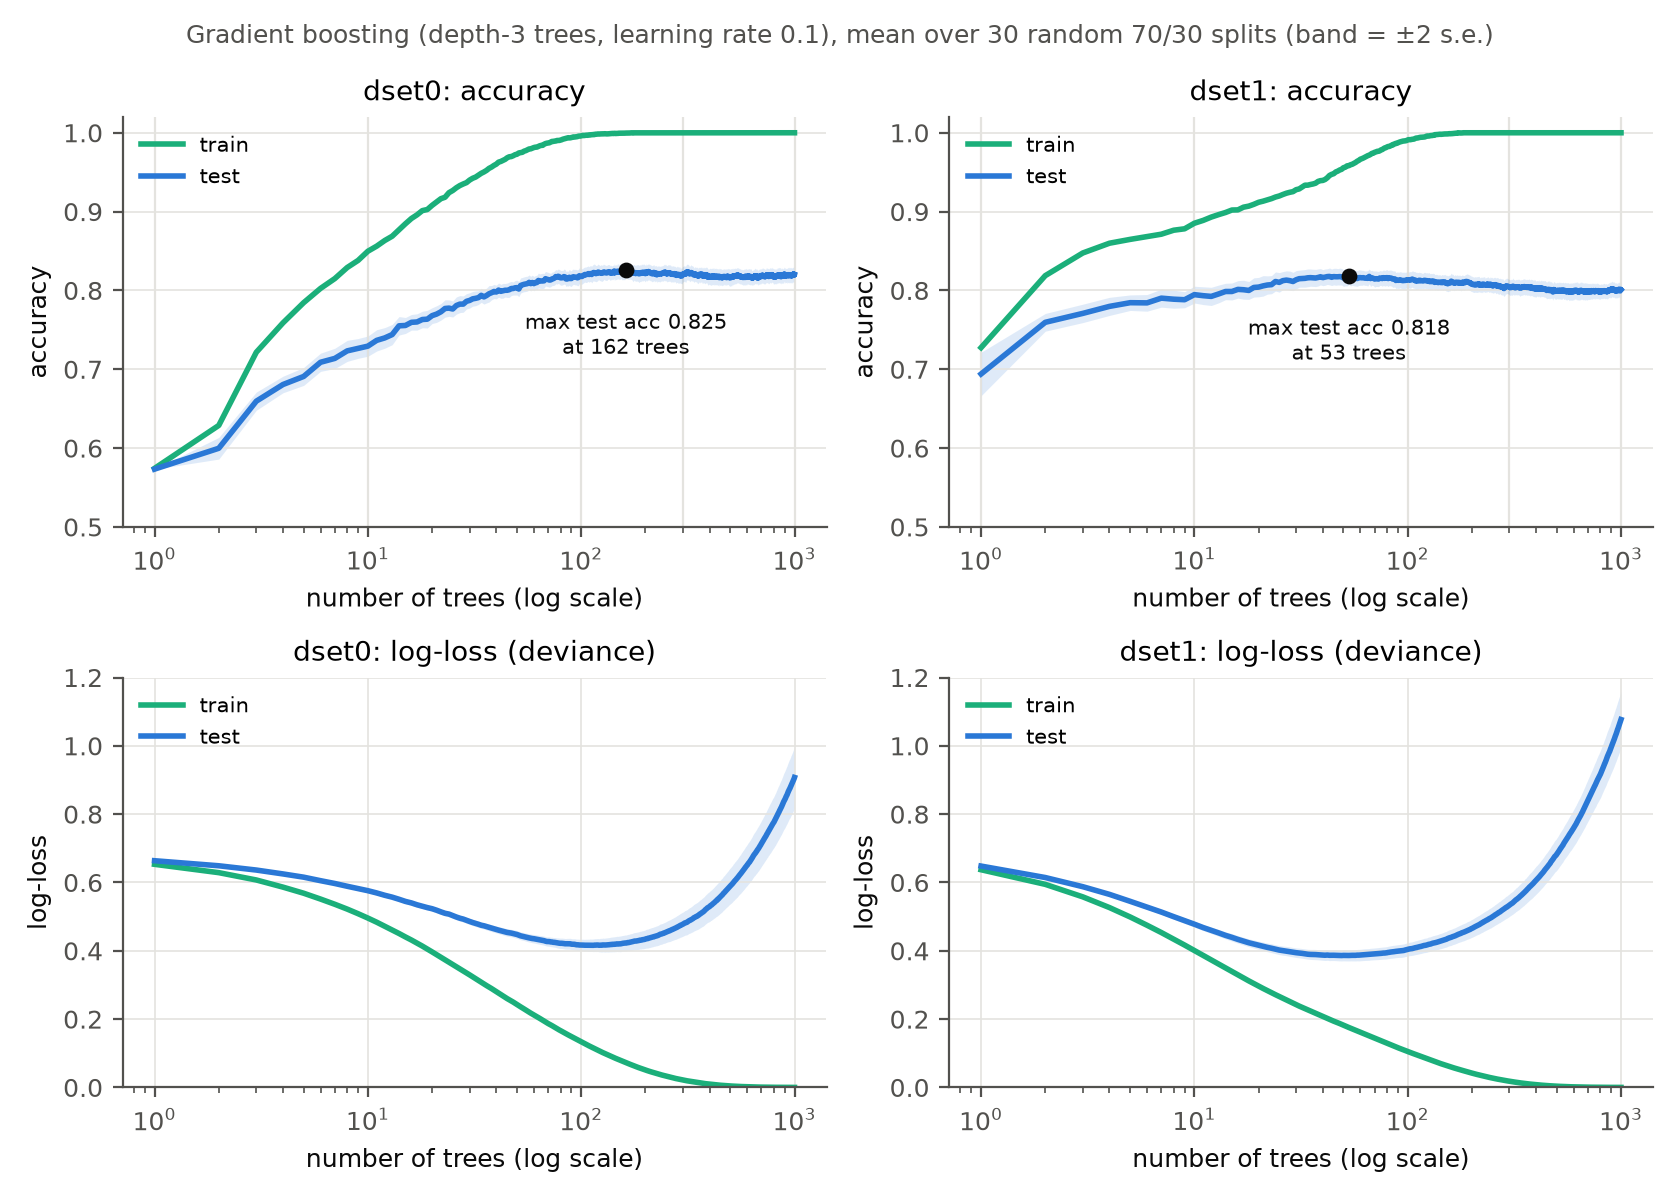
\includegraphics[width=\textwidth]{problem3_curves.png}
\caption{Train/test accuracy (top) and log-loss (bottom) after every number of trees from 1 to
1000, averaged over 30 splits. The vertical grid lines mark 1, 10, 100, 300 and 1000 trees, and
the dot marks the maximum of the mean test accuracy.}
\label{fig:curves}
\end{figure}

\begin{table}[H]\centering\small
\begin{tabular}{lccc}
\toprule
change in test accuracy (same split) & dset0 & dset1\\
\midrule
10 $\to$ 100 trees   & $+0.088\pm0.006$ & $+0.019\pm0.005$\\
100 $\to$ 300 trees  & $+0.003\pm0.003$ & $\mathbf{-0.010\pm0.003}$\\
100 $\to$ 1000 trees & $+0.002\pm0.003$ & $\mathbf{-0.012\pm0.003}$ \ (worse in 20/30 splits)\\
300 $\to$ 1000 trees & $-0.000\pm0.003$ & $-0.003\pm0.002$\\
\bottomrule
\end{tabular}
\caption{Paired differences over the 30 splits (mean $\pm$ standard error). Comparing the
\emph{same} split at two numbers of trees removes most of the split-to-split noise.}
\label{tab:paired}
\end{table}

%==========================================================================
\section*{(a) dset0}

\begin{itemize}
\item \textbf{1 tree} gives the majority-class rate ($0.573$). With learning rate $0.1$, a single
tree moves the log-odds only slightly away from the prior, so no prediction crosses $1/2$.
\item \textbf{1 $\to$ 100 trees.} Test accuracy rises steadily, from $0.729$ at 10 trees to
$0.818$ at 100. Each tree adds real structure.
\item \textbf{100 $\to$ 1000 trees: no overfitting in accuracy.} Training accuracy reaches $1.000$
in every split by about 170 trees, and the training log-loss goes to $0$. The model then fits the training set
perfectly, but test accuracy does \emph{not} get worse: $0.818\to0.820\to0.820$. The paired change
from 100 to 1000 trees is $+0.002\pm0.003$, which is zero. This is the behaviour discussed in
class. Once all training points are classified correctly, further rounds mostly increase the
margins (the confidence) on points that are already correct. The decision boundary barely moves,
so the test error stays where it is even though the model keeps getting more complex.
\item \textbf{The probabilities do overfit.} Test log-loss is smallest at about 110 trees
($0.416$) and then more than doubles, to $0.907$ at 1000 trees. The model becomes extremely
confident, and the few test points it gets wrong are heavily penalized. So ``boosting does not
overfit'' holds here for the \emph{classification decision}, not for the predicted probabilities.
\item With stumps (depth 1, see Figure~\ref{fig:zoom}) dset0 is still \emph{under}fit at 1000 trees.
Test accuracy is $0.797$ and still rising ($+0.018\pm0.004$ from 300 to 1000 trees). An
additive model of single-feature stumps cannot represent the interactions this boundary needs.
\end{itemize}

%==========================================================================
\section*{(b) dset1}

\begin{itemize}
\item \textbf{Fast start.} The signal is picked up much faster than in dset0. Test accuracy is
already $0.795$ with 10 trees (dset0: $0.729$). The mean test accuracy peaks at about \textbf{50
trees} ($0.818$).
\item \textbf{Then it overfits.} After the peak, test accuracy \emph{decreases} as trees are added:
$0.813$ at 100, $0.804$ at 300 and $0.801$ at 1000 trees. The paired drop from 100 to 1000 trees
is $-0.012\pm0.003$, about four standard errors, and 1000 trees are worse than 100 in two thirds of
the splits. Training accuracy is again $1.000$, so the extra trees are fitting something in the
training set that does not carry over to the test set.
\item \textbf{The probabilities overfit even more.} Test log-loss is smallest at about 50 trees
($0.386$) and reaches $1.077$ at 1000 trees.
\item \textbf{Simpler is better here.} Boosted stumps do better than depth-3 trees on dset1
($0.834$ at 300 stumps, Figure~\ref{fig:zoom}). Plain logistic regression does just as well
($0.830$ 5-fold CV accuracy, Table~\ref{tab:diag}). The extra flexibility of deeper trees buys
nothing on this data set.
\item The single split in Table~\ref{tab:single} shows the same pattern (best at 100 trees, worse
afterwards), but the differences there ($0.840$ vs.\ $0.820$/$0.827$) are within the noise of 150
test points. That is why the repeated splits are needed for a reliable conclusion.
\end{itemize}

\begin{figure}[H]\centering
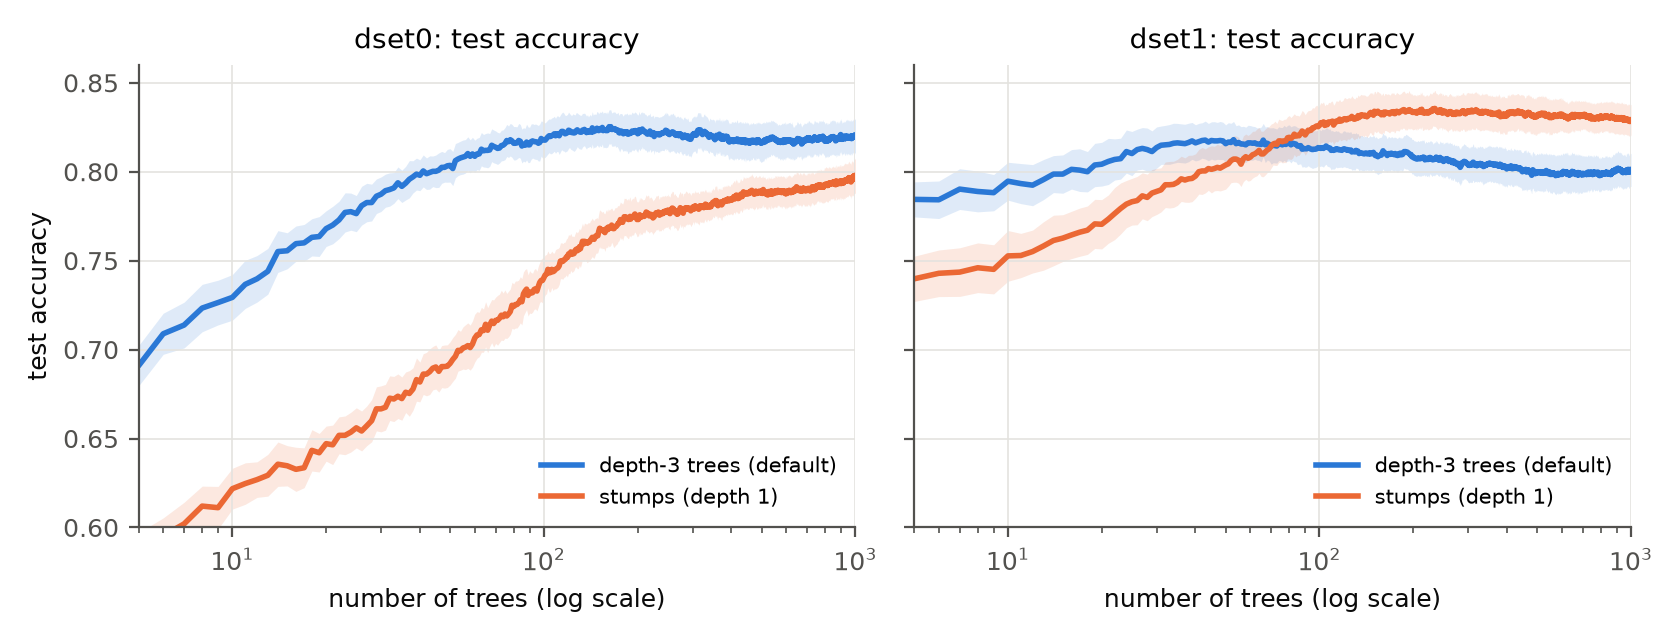
\includegraphics[width=\textwidth]{problem3_test_acc_zoom.png}
\caption{Test accuracy (zoomed, mean $\pm2$ s.e.\ over 30 splits) for depth-3 trees and stumps.}
\label{fig:zoom}
\end{figure}

%==========================================================================
\section*{(c) What property of the data explains the difference?}

\textbf{The amount of label noise relative to the complexity of the true decision boundary.}
dset0 has a complicated, nonlinear boundary and comparatively little label noise. dset1 has a
simple, nearly linear boundary and a lot of label noise (overlapping classes), roughly $17\%$.
The evidence:

\begin{table}[H]\centering\small
\begin{tabular}{lcc}
\toprule
5-fold CV accuracy & dset0 & dset1\\
\midrule
majority class                     & 0.574 & 0.546\\
logistic regression (linear)       & 0.646 & \textbf{0.830}\\
RBF-SVM ($C=10$)                   & 0.828 & 0.790\\
random forest (500 trees)          & \textbf{0.832} & \textbf{0.830}\\
gradient boosting (100 trees)      & 0.822 & 0.808\\
\bottomrule
\end{tabular}
\caption{How much of the signal is linear?}
\label{tab:diag}
\end{table}

\begin{enumerate}
\item \textbf{Shape of the signal (Table~\ref{tab:diag}).} On dset0 a linear model is far behind
the flexible models ($0.646$ vs.\ $\approx0.83$), and boosted stumps underfit. The boundary is
nonlinear and involves interactions. On dset1 logistic regression matches the best flexible model,
and nothing exceeds $\approx83\%$. The Bayes boundary is close to linear, and about $17\%$ of the
labels look irreducibly ``wrong'': the logistic-regression prediction disagrees with $17.6\%$ of
the given labels.

\item \textbf{Where the remaining error comes from (learning curves, Figure~\ref{fig:lc}).} On
dset0 the flexible models are still improving quickly at $n=400$ ($0.81\to0.83$ from 300 to 400
training points). Their error is mostly \emph{estimation/approximation error}: there is more
signal to learn than 350 points reveal. On dset1 logistic regression reaches $0.83$ with only 100
training points and stays flat. Its error is \emph{noise-limited}, and more data or more capacity
cannot remove it.

\item \textbf{Controlled experiments (Figure~\ref{fig:noise}).} Changing \emph{only} the label
noise switches the behaviour:
\begin{itemize}
\item Flipping $20\%$ of dset0's \emph{training} labels (test labels kept clean) makes dset0 behave
like dset1. The test accuracy peaks at 48 trees ($0.73$) and then falls to $0.702$ at 1000 trees.
\item ``Denoising'' dset1, by replacing its labels with the logistic-regression prediction, gives
the same nearly linear boundary with no noise. Boosting then no longer overfits: test accuracy is
$0.908$ at 100 trees, $0.911$ at 300 trees and $0.907$ at 1000 trees, with the maximum at about 300
trees.
\end{itemize}
\end{enumerate}

\paragraph{Mechanism.} Gradient boosting keeps reducing the training log-loss, so it keeps
working on whichever training points are still badly fit.
\begin{itemize}
\item In \textbf{dset0} those points are hard because the boundary is complicated. Fitting them
means learning real structure, which generalizes, so test accuracy rises up to about 100--150 trees.
After the training set is separated, further trees mostly increase margins on correctly classified
points, which leaves the test error unchanged. This is the margin explanation of boosting from
class.
\item In \textbf{dset1} the remaining hard points are mostly \emph{mislabelled}: they sit on the
wrong side of a simple boundary. The only way to fit them is to carve small regions around
individual noisy points. That bends the boundary in ways that are wrong for new data, so test
accuracy falls. The model is also forced to have small margins on exactly those points, so the
margin argument gives no protection.
\end{itemize}
In short, boosting is resistant to overfitting when the training labels are (close to) a
deterministic function of $X$, and it overfits when a substantial fraction of the labels is noise.
In practice the number of trees should therefore be chosen by early stopping on a validation set
(Problem 2), possibly with smaller learning rate, subsampling or shallower trees. Note that the
log-loss overfits on \emph{both} data sets, so early stopping matters whenever calibrated
probabilities are needed.

\emph{Caveat.} dset0's error of about $18\%$ at $n=350$ is not necessarily all approximation error.
Some of it may be noise too. The claim is relative: compared with how complex its signal is, dset0
is much less noisy than dset1.

\begin{figure}[H]\centering
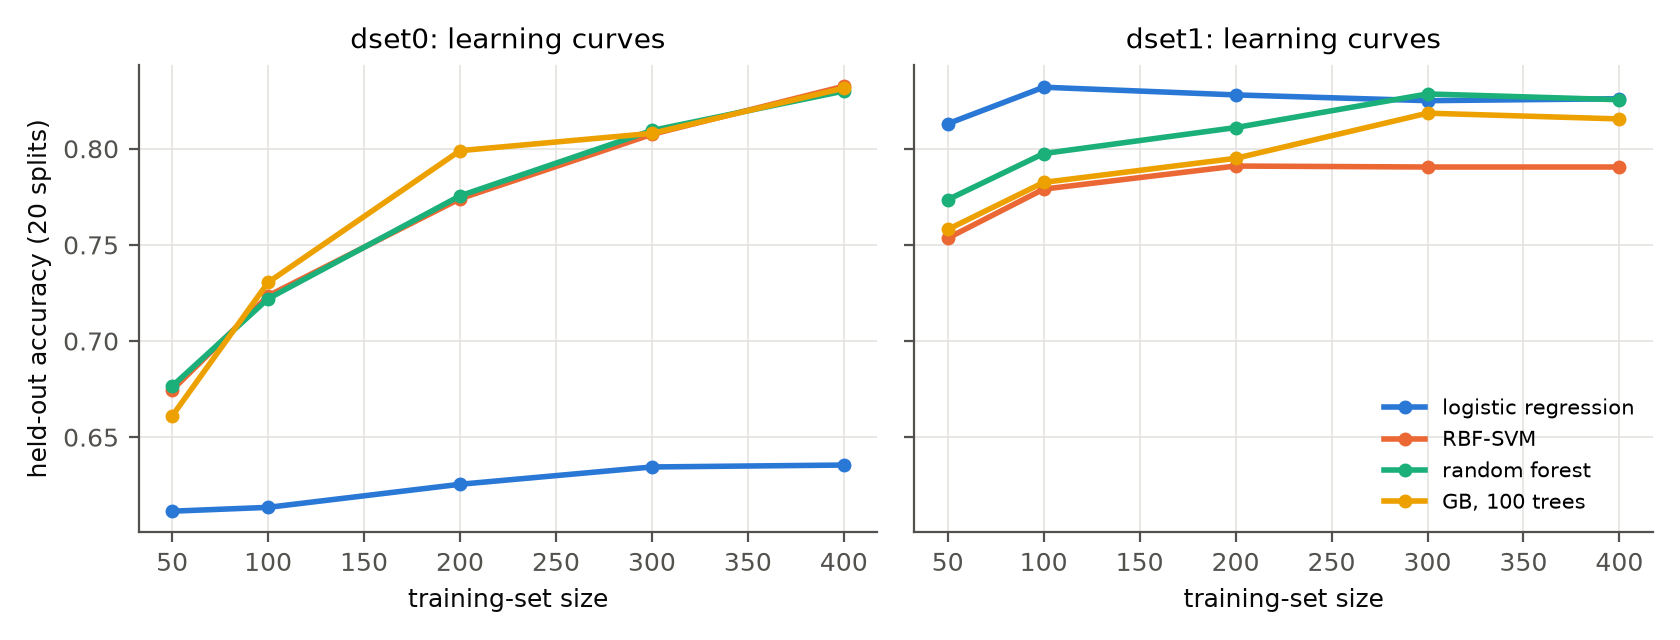
\includegraphics[width=\textwidth]{problem3_learning_curves.png}
\caption{Held-out accuracy vs.\ training-set size (20 random 80/20 splits; training subsets of the
80\%).}
\label{fig:lc}
\end{figure}

\begin{figure}[H]\centering
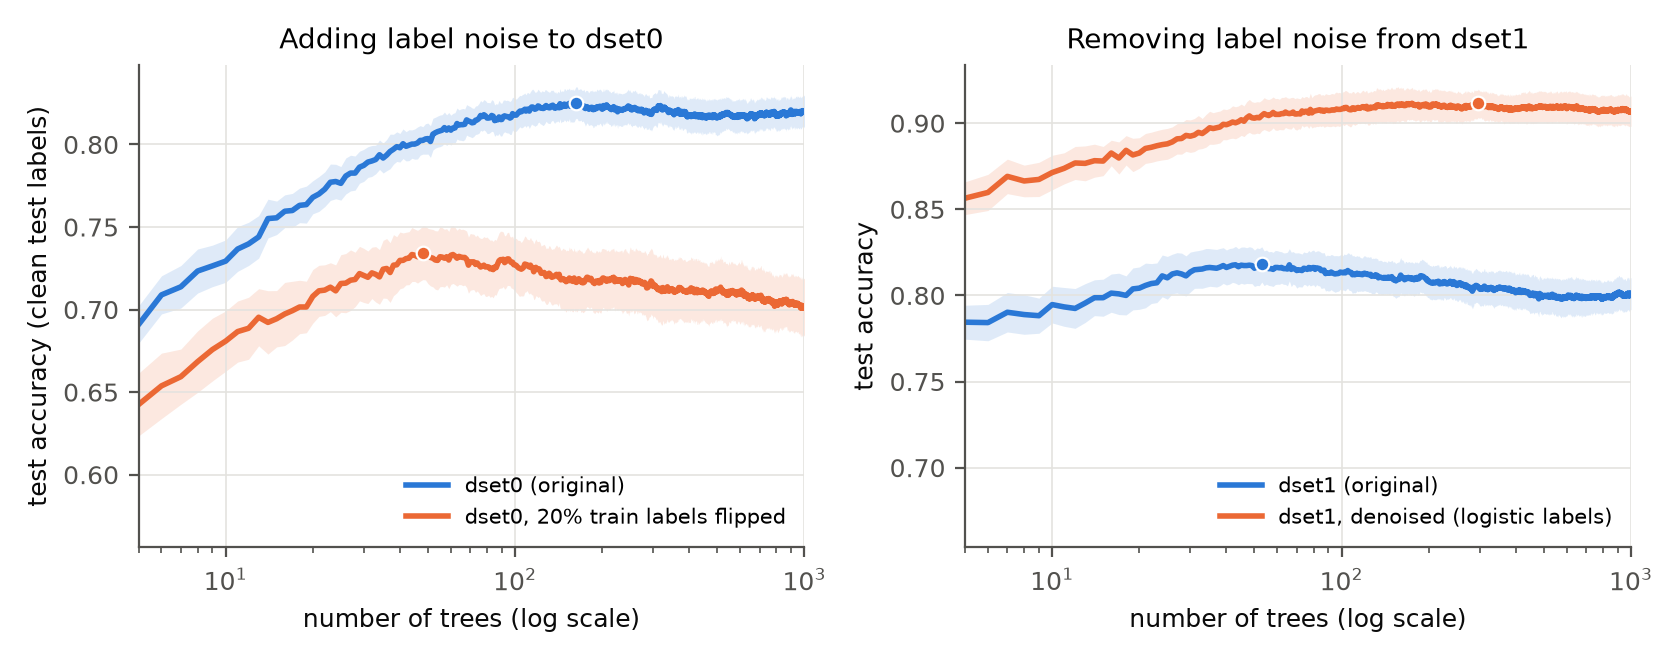
\includegraphics[width=\textwidth]{problem3_label_noise.png}
\caption{Label-noise experiments (30 splits each, mean $\pm2$ s.e.). The dots mark the maximum of
each mean curve.}
\label{fig:noise}
\end{figure}

\end{document}
